\documentclass[12pt]{article}
\usepackage{amsmath}
\usepackage{amssymb}
\usepackage{cancel}
\usepackage{enumitem}
\usepackage{esdiff}
\usepackage{graphicx}
\usepackage{siunitx}
% \usepackage{pgfplots}
\usepackage{wrapfig}

\newcommand{\e}[1]{e^{i(#1)}}
\newcommand{\E}[1]{\times 10^{#1}}

\title{
    Worksheet \#11
    \\  \small
    PHYS 4C: Waves and Thermodynamics
    }
\author{Donald Aingworth IV}
\date{November 3, 2025}

\begin{document}
    \DeclareSIUnit{\celsiusdegree}{C^\circ}
    \DeclareSIUnit{\atm}{ atm}

    \maketitle

    \setcounter{section}{0}
    \section{Problem 1}
        Two sound sources are placed at (0, +1.25 m, 0) and (0, -1.25 m, 0). 
        They both emit isotropic sound waves with a wavelength of 1.00 m at the same total power and in phase with one another. 
        Let I represent the intensity of the sound wave emitted by either source by itself at 100 m distance.

        \subsection{Part (a)}
            As a multiple of I, determine the intensity of the combined sound waves at $(100\,\unit{\meter}, 0, 0)$, $(0, 100\,\unit{\meter}, 0)$ and $(100/\sqrt{2}\,\unit{\meter}, 100/\sqrt{2}\,\unit{\meter}, 0)$. 
            For this part, you may assume that the amplitude of each individual wave is equal to what it would be at 100 m distance.

            \subsubsection{Solution}
                Suppose we call the point at (0, +1.25 m, 0) $r_1$ and the point at (0, -1.25 m, 0) $r_2$.
                First, we do $(100\,\unit{\meter}, 0, 0)$.
                Note the distances between $(100\,\unit{\meter}, 0, 0)$ and both $r_1$ (as $L_1$) and $r_2$ (as $L_2$).
                \begin{gather}
                    L_1 = \sqrt{100^2 + 1.25^2}\\
                    L_2 = \sqrt{100^2 + 1.25^2}\\
                    L_1 = L_2
                \end{gather}

                The two waves travel an identical distance, so they will be in phase. 
                This means that the amplitude will be the amplitude of the other two waves added together (in this case doubling).
                Since $I \varpropto A^2$, the intensity will in turn quadruple, leaving us with a final intensity of $4I$.

                Second, we do $(0, 100\,\unit{\meter}, 0)$. 
                We can calculate $\Delta L$ directly.
                \begin{equation}
                    \Delta L = 1.25\,\unit{\meter} + 1.25\,\unit{\meter} = 2.50\,\unit{\meter}
                \end{equation}

                Take the modulus of this with respect to the wavelength ($\lambda = 1$).
                \begin{equation}
                    \Delta L \equiv 0.5 \mod \lambda
                \end{equation}

                Divide both sides by the wavelength.
                \begin{equation}
                    \frac{\Delta L}{\lambda} \equiv 0.5 \mod 1
                \end{equation}

                Ths means that the difference $\Delta \phi = \pi$, so there is destructive interference.
                This means that the amplitudes added together would be equal to zero.
                In turn, the resultant intensity would be equal to 0.

                Lastly, we do $(100/\sqrt{2}\,\unit{\meter}, 100/\sqrt{2}\,\unit{\meter}, 0)$. 
                Calculate the values of $L_1$ and $L_2$.
                \begin{gather}
                    L_1 = \sqrt{\left( \frac{100}{\sqrt{2}} + 1.25 \right)^2 + \left( \frac{100}{\sqrt{2}} \right)^2}\\
                    L_2 = \sqrt{\left( \frac{100}{\sqrt{2}} - 1.25 \right)^2 + \left( \frac{100}{\sqrt{2}} \right)^2}
                \end{gather}

                Subtract $L_2$ from $L_1$ to find the change in distance.
                \begin{align}
                    \Delta L    &=  L_1 - L_2\\
                        &=  \sqrt{\left( \frac{100}{\sqrt{2}} + 1.25 \right)^2 + \left( \frac{100}{\sqrt{2}} \right)^2} - \sqrt{\left( \frac{100}{\sqrt{2}} - 1.25 \right)^2 + \left( \frac{100}{\sqrt{2}} \right)^2}\\
                        &=  100.887\,\unit{\meter} - 99.120\,\unit{\meter}
                        =   1.768\,\unit{\meter}
                \end{align}

                Take the modulus of this with respect to the wavelength.
                \begin{equation}
                    \Delta L \equiv 0.768 \mod \lambda
                \end{equation}

                Divide by the wavelength and multiply by $2\pi$ to get $\Delta \phi$.
                \begin{equation}
                    \Delta \phi = \frac{2\pi\,\Delta L}{\lambda}
                        =   2\pi \times 0.768
                \end{equation}
                
                Multiply the initial intensity by four, them multiply that by the square of the cosine of this divided by two to get the intensity of the resultant wave.
                \begin{equation}
                    I_3 =   4I\cos^2\left( 0.768\pi \right)
                        =   2.22I
                \end{equation}

                Conclusively, here are our values.
                \begin{center}
                    \begin{tabular}{|c|c|}
                        \hline
                        \textbf{$\vec{r}$} & \textbf{I($\vec{r}$)}\\
                        \hline
                        $(100\,\unit{\meter}, 0, 0)$ & $4I$\\
                        \hline
                        $(0, 100\,\unit{\meter}, 0)$ & $0$\\
                        \hline
                        $(100/\sqrt{2}\,\unit{\meter}, 100/\sqrt{2}\,\unit{\meter}, 0)$ & $2.22I$\\
                        \hline
                    \end{tabular}
                \end{center}

        \subsection{Part (b)}
            If you were to walk along a 90\unit{\degree} arc in the x-y plane between (100 m, 0, 0) and (0, 100 m, 0), how many interference maxima would you encounter?
            Interference minima?

            \subsubsection{Solution}
                Assume the arc to be a circular arc.
                Also call the distance between the two points (2.50 m) $D$.
                We are looking for cases where the remainder of $\frac{\Delta L}{\lambda}$ and 1 is 0.5.
            \begin{equation}
                \frac{\Delta L}{\lambda} \equiv 0.5 \mod 1
            \end{equation}

            Suppose that the radius of the circle is $R$.
            This would create two vectors, once for the distance from $S_1$ and $S_2$.
            \begin{align}
                &\vec{L}_1  =   R\begin{pmatrix}
                    \cos(\theta) + \frac{D}{2}\\
                    \sin(\theta)
                \end{pmatrix}
                &\vec{L}_2  =   R\begin{pmatrix}
                    \cos(\theta) - \frac{D}{2}\\
                    \sin(\theta)
                \end{pmatrix}
            \end{align}

            From this, we can create a formula for $\Delta L$ and graph it on a plane.
            \begin{align}
                \left| \left| L_1 \right| \right|   &=  \sqrt{\left( \cos(\theta) + \frac{D}{2} \right)^2 + \sin^2(\theta)}\\
                \left| \left| L_2 \right| \right|   &=  \sqrt{\left( \cos(\theta) - \frac{D}{2} \right)^2 + \sin^2(\theta)}\\
                \Delta L    &=  \sqrt{\left( \cos(\theta) - \frac{D}{2} \right)^2 + \sin^2(\theta)} - \sqrt{\left( \cos(\theta) + \frac{D}{2} \right)^2 + \sin^2(\theta)}
            \end{align}
            \begin{center}
                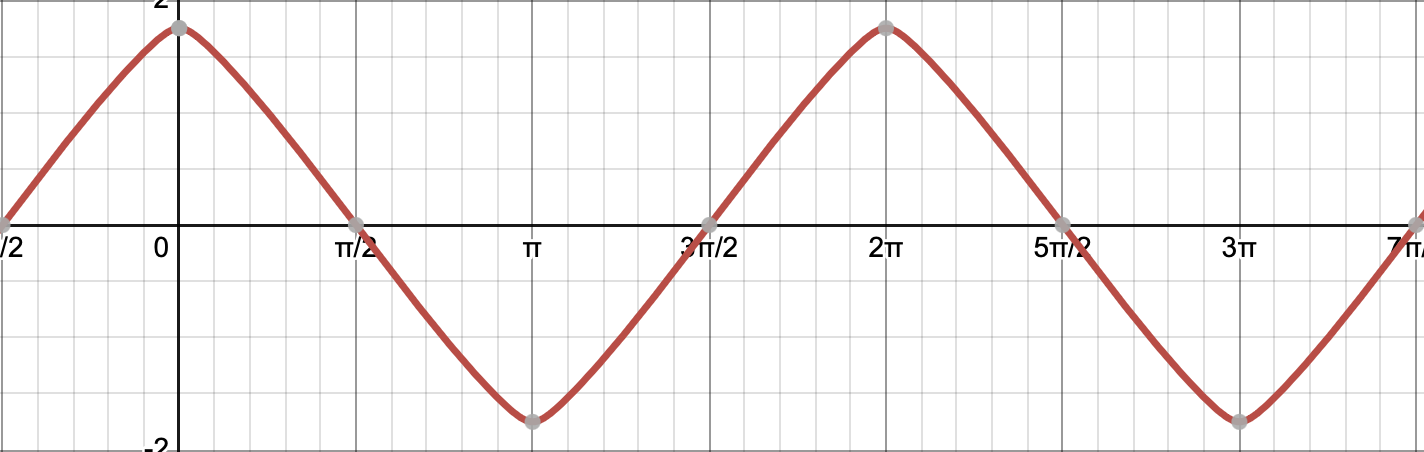
\includegraphics[width=\textwidth]{Fig-19-1.png}
            \end{center}

            Looking at it here, we can see that between 0 and $\frac{\pi}{2}$, it does not change direction once.
            Knowing this, we can first calculate the variation in the value of $\Delta L$.
            This applies for between when $\theta = 0$ and $\theta = \frac{\pi}{2}$.
            \begin{align}
                \Delta L(0) &=  \sqrt{\left( \cos(0) - \frac{D}{2} \right)^2 + \sin^2(0)} - \sqrt{\left( \cos(0) + \frac{D}{2} \right)^2 + \sin^2(0)}\\
                    &=  \sqrt{\left( \cos(0) - \frac{D}{2} \right)^2} - \sqrt{\left( \cos(0) + \frac{D}{2} \right)^2}
                    =   -D\\
                \Delta L\left( \frac{\pi}{2} \right)    &=  \sqrt{\left( \frac{D}{2} \right)^2 + \sin^2(0)} - \sqrt{\left( \frac{D}{2} \right)^2 + \sin^2(0)}
                    =   0
            \end{align}

            In any case, we would only have to find the points at which $\frac{\Delta L}{\lambda} \equiv 0.5 \mod 1$ for $0 \leq \Delta L \leq D$.
            Since $\lambda = 0.5$, dividing everything by $\lambda$ would be equivalent to multiplying by 2, so we can use that for the limits.
            \begin{gather}
                0 \leq \Delta L \leq D\\
                0 \leq \frac{\Delta L}{\lambda} \leq 2D\\
                0 \leq \frac{\Delta L}{\lambda} \leq 2.5
            \end{gather}

            At this point, we could just count the cases that work for the requirements.
            If one of the boundary cases applies, we should only consider it as half of a case that works.
            \begin{center}
                1: $0 \leq 0.5 \leq 2.5$;
                2: $0 \leq 1.5 \leq 2.5$;
                3: $0 \leq 2.5 \leq 2.5$
            \end{center}
            This leaves us with two and a half interference maxima in the first quarter of the circle.

            For the interference minima, it would instead be $\frac{\Delta L}{\lambda} \equiv 0.5 \mod 1$.
            Time to count.
            \begin{center}
                1: $0 \leq 0 \leq 2.5$;
                2: $0 \leq 1 \leq 2.5$;
                3: $0 \leq 2 \leq 2.5$
            \end{center}

            This also lands us with two and a half cases of interference maxima.

        \subsection{Part (c)}
            Now take into account the fact that the sound sources are not exactly 100 m away from the point (0, 100 m, 0) and the impact that has on the amplitude of the individual sound waves, and calculate the intensity of the combined wave at that point.

            \subsubsection{Solution}
                First calculate the exact amplitude of the waves at that point.
                The intensity of a sound wave at a point is calculatable by dividing the powe by the area.
                In this case, the area is equal to the surface area of a sphere ($4\pi r^2$).
                \begin{equation}
                    I = \frac{P}{A} = \frac{P}{4\pi r^2}
                \end{equation}

                Here, the only thing the does not change is the power (besides the $4\pi$, but that's neither here nor there).
                We can create two separate cases and compare those two cases.
                \begin{gather}
                    I_1 = \frac{P}{4\pi r_1^2}\\
                    I_2 = \frac{P}{4\pi r_2^2}\\
                    I_1 r_1^2 = \frac{P}{4\pi} = I_2 r_2^2 \to 
                    I_2 = I_1 \frac{r_1^2}{r_2^2}
                \end{gather}

                We can now consider the case of the intensity from points 1 (for which $r_1 = 101.25\,\unit{\meter}$) and 2 (for which $r_2 = 98.75\,\unit{\meter}$).
                We will have a value of $r_0 = 100\,\unit{\meter}$.
                \begin{align}
                    I_1 &=  I_0 \frac{r_0^2}{r_1^2}
                        =   I_0 \frac{100^2}{101.25^2}
                        =   0.975 I_0\\
                    I_2 &=  I_0 \frac{r_0^2}{r_2^2}
                        =   I_0 \frac{100^2}{98.75^2}
                        =   1.025 I_0
                \end{align}

                They have a previously established destructive interference.
                This means that the resultant amplitude will be the difference between the starting amplitudes.
                The amplitude itself is proportional to the square root of the intensity.
                Suppose that everything but $s_m$ and the initial intensity $I$ are equal to a constant $c$.
                \begin{equation}
                    I = c s_m^2 \to s_m = \sqrt{\frac{I}{c}}
                \end{equation}

                Take the difference of $s_m$ from points 1 and 2.
                \begin{align}
                    s_{net} &=  s_2 - s_1
                        =   \sqrt{\frac{I_2}{c}} - \sqrt{\frac{I_1}{c}}\\
                        &=  \sqrt{\frac{I_0}{c}} \left( \frac{100}{98.75} - \frac{100}{101.25} \right)
                        =   0.025 \sqrt{\frac{I_0}{c}}
                \end{align}

                Square it.
                \begin{equation}
                    s_{net}^2 = 0.025^2 \frac{I_0}{c}
                \end{equation}

                Multiply by the constant $c$ from prior.
                You will find you will get the net intensity at the point.
                \begin{equation}
                    I_{net} =   0.025^2 I
                        =   \boxed{6.25\E{-4} I}
                \end{equation}

    \pagebreak
    \section{Problem 2}
        Two opera singers (standing still) are singing a high A (f = 880 Hz) and low A (f = 220 Hz), respectively, when a car carrying a sound-reflecting wall is travelling towards them at 0.100 times the speed of sound. 
        Determine the frequencies of the reflected sound waves, as would be heard by the opera singers.
        
        Note: No opera singers were harmed during the construction of this question or its solution.

        \subsection{Solution}
            The car as a detector is effectively traveling towards the source at a speed of the speed of the car.
            \begin{align}
                f'  &=  f\frac{v_s + 0.1 * v_s}{v_s}
                    =   f * 1.1
            \end{align}

            Furthermore, the singers as detectors would be receiving sound from the car moving at the speed of the car.
            \begin{align}
                f'' &=  f'\frac{v_s}{v_s - 0.1 * v_s}
                    =   f' * \frac{10}{9}
                    =   f * 1.1 * \frac{10}{9}
                    =   f * 1.\bar{2}
            \end{align}

            The high A (1) and low A (b) would be accordingly calculatable.
            \begin{align}
                f'_1 &= f_1 * 1.\bar{2} = 880\unit{\hertz} * 1.\bar{2} = \boxed{1075.\bar{5}\unit{\hertz}}\\
                f'_2 &= f_2 * 1.\bar{2} = 220\unit{\hertz} * 1.\bar{2} = \boxed{268.\bar{8}\unit{\hertz}}
            \end{align}
\end{document}